\section{Preliminary and Related Works}
\label{sec:Preliminary}
\subsection{SystemVerilog Assertions}
\label{subsec:SVA}
An SVA is constructed using different signals from the hardware design, that are then composed using various \textit{SVA operator}s to describe functional or temporal relationships between signals.
In SystemVerilog, there are two kinds of assertions: \textit{immediate assertions} and \textit{concurrent assertions}~\cite{IEEEStd}.
% , both of which can be invoked with the \verb|assert| keyword.. 

Immediate assertions execute  within procedural code (for example, inside an \verb|initial|/\verb|always| block). 
They check combinational conditions using \textit{Boolean operator}s such as \texttt{!}, \texttt{\&\&}, and \texttt{||}, serving as runtime self-checks during simulation.
For example:
\begin{verbatim}
     assert (valid && (req || grant));
\end{verbatim}
It checks the combinational condition that signal \verb|valid| is true, and at least one of signal \verb|req| or signal \verb|grant| is true.

A concurrent assertion used to specify temporal properties of a design is constructed in four hierarchical layers~\cite{IEEEStd}. 
\begin{itemize}
    \item \textit{Boolean Layer}: that combines signals using Boolean operators, as noted above.
    \item \textit{Sequence Layer}: that applies \textit{Sequence Operator}s to one or more combinational expressions obtained from the Boolean layer. Sequence operators are shown in Table~\ref{tab:sequence_sva_operators}.
    % by applying \textit{Sequence SVA Operator}s to one or more combinational expressions.
    \item \textit{Property Layer}: that applies \textit{Property Operator}s, shown in Table~\ref{tab:property_sva_operators}, to one or more sequential expressions.
    % by applying \textit{Property SVA Operator}s to one or more sequence expressions.
    \item \textit{Verification Layer}: that binds a property expression to the design’s clock and reset signals, and wrap it in an \texttt{assert property (...)} directive.
\end{itemize}
Each SVA operator may take one or two operands. An operator introduced at a layer accepts operands that are expressions of that layer or of the layer immediately below it. Table~\ref{tab:sequence_sva_operators} shows $7$ types of sequence SVA operators and Table~\ref{tab:property_sva_operators}  shows $3$ types of property SVA operators.
%The two tables include the usage and explanation of ea.
% Concurrent assertions are used to specify temporal properties of a design. 
% Unlike immediate assertions, concurrent assertions not only use Boolean SVA operators but also temporal SVA operators, such as non-overlapping implication ($|$\verb|->|), overlapping implication ($|$\verb|=>|), and cycle delay (\texttt{\#\#}) to connect signals. 
% % The general format is: 
% % \begin{verbatim}
% % assert property (@posedge(clock_signal) 
% % disable iff(reset_signal) 
% % logical_expression);
% % \end{verbatim}
% % The keyword \verb|property| differentiates a concurrent assertion from an immediate one.
% % The part \verb|@posedge(clock_signal)| specifies the event on which the assertion is evaluated (in this case, the positive edge of a clock signal). 
% % This is optional; if omitted, the assertion is evaluated continuously.
% % The second part \verb|disable iff(reset_signal)| indicates that the assertion should be disabled when a particular condition holds (e.g., when the reset signal is active). 
% % This part is also optional.
% % The last part \verb|logical_expression| represents the property to be checked, constructed using Verilog signals and SVA syntaxes. 
% % A concurrent assertion is built on the notion of a \textit{property}, which can include sequences with temporal operators. 
% Its general format is: 
% \begin{verbatim}
% assert property (@posedge(clock_signal) 
% disable iff(reset_signal) 
% logical_expression);
% \end{verbatim}
% The keyword \verb|property| differentiates a concurrent assertion from an immediate one.
% The part \verb|@posedge(clock_signal)| specifies the event on which the assertion is evaluated (in this case, the positive edge of a clock signal). 
% This is optional; if omitted, the assertion is evaluated continuously.
% The second part \verb|disable iff(reset_signal)| indicates that the assertion should be disabled when a particular condition holds (e.g., when the reset signal is true). 
% This part is also optional.
% The last part \verb|logical_expression| represents the property to be checked, constructed using Verilog signals and SVA operators. 
Fig.~\ref{fig:four-layers-sva} shows an example of an SVA, where all expressions in the four layers are marked using boxes with different colors.
\begin{figure}
    \centering
    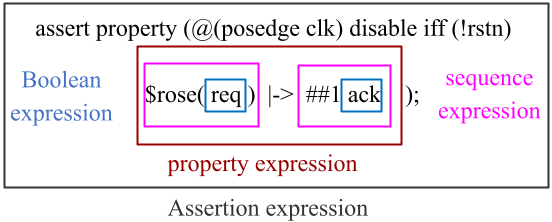
\includegraphics[width=0.65\linewidth]{Figs/FourLayersSVA.png}
    \caption{Four layers of an example concurrent assertion.}
    \label{fig:four-layers-sva}
\end{figure}
% In the following, an example concurrent assertion is shown:
% \begin{verbatim}
%     assert property (
%         @(posedge clk) disable iff (!rstn)
%         $rose(req) |-> ##1 ack
%     );   
% \end{verbatim}
% At the Boolean layer the only combinational expressions are the individual signals \texttt{req} and \texttt{ack}.
% At the sequence layer, there are two sequence expressions. The first is \texttt{\$rose(req)} and the second is \texttt{\#\#1} ack.
% In the Property layer, those two sequence expressions are combined by the operator \texttt{|->}, yielding the property expression \texttt{\$rose(req) |-> \#\#1 ack}. 
% In the context of \texttt{|->} and \texttt{|=>}, which are also called \textit{implication operator}s, their first operand is called \textit{precondition} and the second operand is called \textit{consequent}.
% Thus, \texttt{\$rose(req)} is the precondition and \texttt{\#\#1 ack} is the consequent.
% Finally, the verification layer binds the property expression to \texttt{@(posedge clk)} specifying the verification occuring on each rising edge of \texttt{clk}, and the clause disable \texttt{iff (!rstn)} specifying the verification occuring when \texttt{rstn} is $1$, which is futher wrapped by \texttt{assert property()}.
% The non-overlapping implication  $|$\verb|->| connects two parts:
% \begin{itemize}
%     \item the \textit{precondition}, \verb|req|, which specifies the event to monitor at the clock edge;
%     \item the \textit{consequent}, \verb|##1 ack|, which describes the expected behavior following the precondition. 
% \end{itemize}
% Specifically, this assertion specifies that when signal \verb|req| is true at a rising clock edge (precondition), then signal \verb|ack| must be true exactly one clock cycle later (consequent).
% In other words, the assertion does not evaluate the consequent if the precondition is never satisfied.
% % In other words, the assertion will not check the consequent when the precondition can never be true.
% This structure of a precondition and consequent also applies to the overlapping implication operator $|$\verb|=>|, although the timing behavior differs slightly.
\begin{table}[t]
\centering
\caption{Sequence SVA Operators}
\label{tab:sequence_sva_operators}
\begin{tabular}{|c|c|}
\hline
\textbf{SVA Operator} & \textbf{Explanation} \\ \hline
\texttt{\#\#N s} & \tabincell{l}{The evaluation of sequence expression \texttt{s} is delayed\\ by \texttt{N} clock cycles.} \\ \hline
\texttt{\$rose(s)} & \tabincell{l}{Returns $1$ if the LSB of sequence expression \texttt{s}\\ changed to $1$. Otherwise, returns $0$.} \\ \hline
\texttt{\$fell(s)} & \tabincell{l}{Returns $1$ if the LSB of sequence expression \texttt{s}\\ changed to $0$. Otherwise, returns $0$.} \\ \hline
\texttt{\$past(s,N)} & \tabincell{l}{Returns the value of sequence \texttt{s} in a \texttt{N} clock cycle \\step prior to the current one.} \\ \hline
\texttt{\$stable(s)} & \tabincell{l}{Returns $1$ if the value of sequence expression \texttt{s}\\ did not change. Otherwise, returns $0$.} \\ \hline
\texttt{\$onehot(s)} & \tabincell{l}{Returns $1$ if one bit of sequence expression \texttt{s}\\ is $1$. Otherwise, returns $0$.} \\ \hline
\texttt{\$onehot0(s)} & \tabincell{l}{Returns $1$ if no more than one bit of sequence\\ expression \texttt{s} is $1$. Otherwise, returns $0$.} \\ \hline
\end{tabular}
\end{table}

\begin{table}[t]
\centering
\caption{Property SVA Operators}
\label{tab:property_sva_operators}
\begin{tabular}{|c|c|}
\hline
\textbf{SVA Operator} & \textbf{Explanation} \\
\hline
\texttt{s |-> p} & \tabincell{l}{for every match of the sequence expression \texttt{s} \\beginning at the start point, the evaluation of\\ property expression \texttt{p} beginning in the current\\ clock cycle at the end point of the match \\succeeds and returns $1$.} \\ \hline
\texttt{s |=> p} & \tabincell{l}{for every match of the sequence expression \texttt{s} \\beginning at the start point, the evaluation of\\ property expression \texttt{p} beginning in the next\\ clock cycle at the end point of the match \\succeeds and returns $1$.} \\ \hline
\texttt{s\_eventually p} & \tabincell{l}{Return $1$ if there exists a current or future clock \\cycle at which property expression \texttt{p} is $1$.} \\ \hline
\end{tabular}
\end{table}

\subsection{Retrieval-Augmented Generation}
\label{subsec:RAG}
RAG is a technique that enhances the performance of LLMs by incorporating relevant external knowledge~\cite{Lewis20}.
%, especially on domain-specific tasks. 
Instead of relying solely on the LLM's internal knowledge, RAG augments the model’s input by retrieving relevant external documents from a knowledge database based on the query.
RAG has been successfully applied in different fields, such as code generation~\cite{Koziolek24}, medical QA~\cite{xiong2024}, financial QA~\cite{Setty24}, and conversational agents~\cite{alonso2024}.
% In Fig.~\ref{fig:Flow-of-Basic-RAG}, it shows the flow of basic RAG, which consists of two key components. 

RAG methods leverage a specialized database of \textit{vector embeddings}, created by first splitting the source materials, such as documents or code repositories, into smaller \textit{chunks} and then transforming each chunk into a numerical representation using an embedding model, i.e., a vector embedding. 
% By storing these embeddings as indexes in the database, the system can efficiently retrieve relevant information based on \textit{similarity search} when it receives a user’s input prompt.
The strategy used for splitting the source materials significantly impacts the relevance of retrieved chunks to the input prompt. 
A common practice is to apply \textit{static splitting}, where the source data is divided into fixed-size text chunks, typically based on a constant number of characters. 
A common method for enhancing the static splitting techniques is to employ LLM-based splitting, which leverages LLMs to identify more semantically coherent chunk boundaries~\cite{singh24,chang24n,dong24}.
However, they require careful prompt design and substantial computational overhead.
%While simple to implement, static splitting often ignores semantic boundaries in the content, separating logically related information across different chunks and thereby degrading retrieval quality.

The \textit{retrieval process}, which serves as the second key component of RAG, begins with an input prompt.
% As is shown in Fig.~\ref{fig:Flow-of-Basic-RAG}, the \textit{retrieval process}, which is the other key part of RAG, begins with an \textit{initial prompt}, which can be a question, an instruction, or another form of request for information. 
This prompt is transformed into a vector embedding using the same embedding model for constructing the database.
Then, the retrieval process uses \textit{similarity search} to identify the top-ranked or most similar chunks that align with the the input prompt, returning them as the \textit{relevant context}.
The original input prompt is then augmented with the relevant context to form a \textit{combined prompt}, enriching the LLM with domain-specific knowledge. 
The combined prompt guides the LLM to generate more accurate and context-aware responses. 
% RAG effectively bridges the gap between the model’s internal knowledge and the external information retrieved from the database, leading to informed and reliable results.

% The original prompt is then augmented with this retrieved context to form a \textit{combined promp}t, providing the LLM with direct, domain-specific information that may not be fully captured by its training alone.
% Finally, the combined prompt instructs the LLM to generate more accurate responses.

%The final generation step occurs when the LLM processes the combined prompt and produces a response. 
% Thus, RAG bridges the gap between the model’s internal knowledge, learned during pre-training, and the external knowledge retrieved in the database, leading to more informed and reliable results.

% \begin{figure}
%     \centering
%     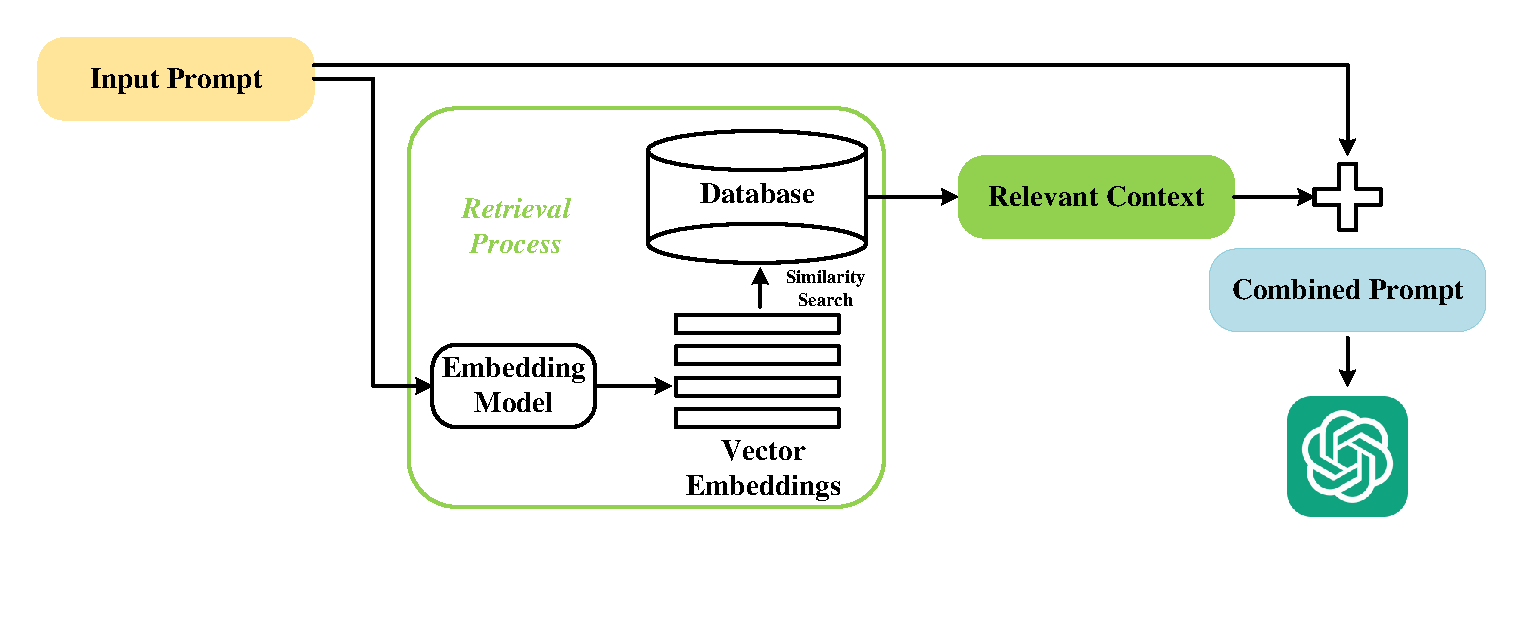
\includegraphics[width=\linewidth]{Figs/Basic_RAG_Flow.pdf}
%     \caption{Flow of basic RAG.}
%     \label{fig:Flow-of-Basic-RAG}
% \end{figure}

\subsection{Related Works}
A critical component for evaluating LLM-based
NL2SVA is the evaluation dataset. 
Prior works such as \textit{AssertionBench}~\cite{Vaishnavi25}, \textit{AssertLLM}~\cite{Yan25}, and \textit{FVEval}~\cite{Minwoo24} have provided open-source
datasets for benchmarking assertion generation. 
However, AssertionBench and AssertLLM lack detailed contextual information, such as natural language explanations of the SVAs.
This missing information is essential for rigorously evaluating
the functionality match between the generated SVAs and their
expected natural language property descriptions. 
FVEval introduces a more comprehensive dataset, containing $13$ hardware
designs, $80$ SVAs with corresponding human-written property
explanations.

